\chapter{Topic modelling}\label{ch:topicmodelling}
Once extensively analysed the structure of the dataset, the goal becomes to develop a machine learning method to learn the hidden structure of the data.  
%%intro
Remembering that in chapter~\ref{ch:structure} it emerged some kind of structure behind data, where each tissue seemed to be sampled by a different power law, a topic modelling approach is here proposed. Topic modelling has been developed and studied to approach linguistics problems, so this algorithm was developed considering words and books in input, links represent the abundance of a word in a book. In chapter~\ref{ch:structure} was evident that there are many similarities between data considered in this work and linguistics' corpora. Referring to data used in this project \textbf{samples} will be the documents and \textbf{genes} will be the words. It is expected that topics represent some properties of the system due to the gene expression distribution in samples.

The idea is that behind data there are hidden variables that describe the relationship between the genes and the samples. Let's call these variables topics.
Firstly it is necessary to build a bipartite network of genes and samples, then nodes are linked considering the gene expression value in the dataset.
\begin{figure}[htb!]
    \centering
    \includegraphics[width=0.7\linewidth]{pictures/topic/bipartite.pdf}
    \caption{An example of a bipartite network. Samples are on the left, genes are on the right. Each link is weighted by gene expression value. On the left side, all nodes of the same colour are clusters of samples. On the right side, all nodes with the same colour are a set of genes, also known as topics.\\
    Blue lines represent the cluster structure, each blue squared-dot is a set of nodes, lines delineate the hierarchical structure.\\
    It is clear in the middle the network separation between genes and samples.}
    \label{fig:topic/bipartite}
\end{figure}

The output of this kind of models consists of sets of genes, the topics, with a probability distribution $P(\text{gene} | \text{topic})$ and probability distributions of these topics inside each sample $P(\text{topic} | \text{sample})$, together they give the relationship between a \textit{sample} and a \textit{gene}.

In this work, an innovative and recent approach to topic model is proposed. The algorithm was presented by~\cite{gerlach2018network} and~\cite{Peixoto2017} explain it in details. This model is an evolution of a stochastic block model~\cite{Holland1983}. It is called hierarchical Stochastic Block Model (hSBM).

The ultimate goal is to be able to separate healthy and diseased samples then find and separate well-known tumour types and finally extend the actual knowledge and retrieve the tumour sub-types.

One of the advantages of this particular algorithm is that it is hierarchical, so it applies community detection at different layers of resolution. So the output has got different resolutions and different number of clusters at each layer . One extreme layer is the one which separates genes ($\simeq$ words) and samples ($\simeq$ samples), by definition; in other layers, it is possible to have few big clusters until the other extreme were the number of clusters is comparable with the number of nodes.
\begin{figure}[htb!]
  \centering
  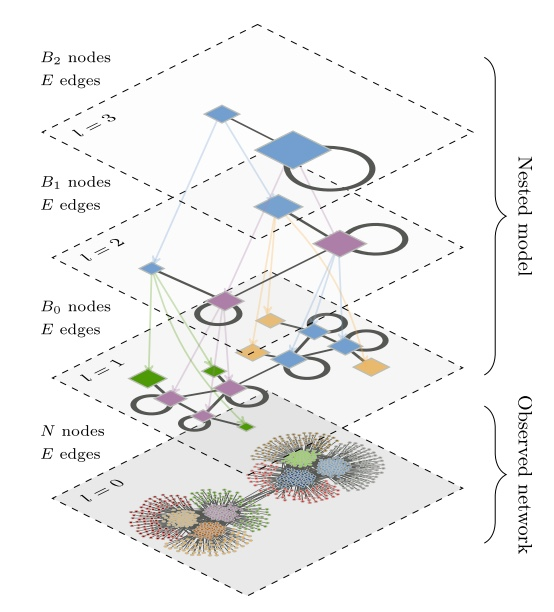
\includegraphics[width=0.6\linewidth]{pictures/topic/peixioto_hierarchic.jpg}
  \caption{Example of a hierarchical structure. At $l=0$ the number of cluster is comparable with the number of nodes, is the situation with many small clusters. Then they're merged in bigger clusters at other layers of the hierarchy.}
  \label{fig:topic_peixioto_hierarchic}
\end{figure}

What the algorithm does is to run a sort of Monte Carlo simulation and find the best partition of the data.
The probability that the hidden variables $\theta$ describe the data $G$ $P(\theta | G)$ can be written as a likelihood times a prior probability as
\[P(\theta|G)=\frac{P(G|\theta)\overbrace{P(\theta)}^{prior}}{\underbrace{P(G)}_{\sum_{\theta}P(G|\theta)P(\theta)}}.\]
It is possible to define a description length
\[
\Sigma=-lnP(G|\theta)-lnP(\theta),
\]
so that $P(\theta | G)\propto e^{-\Sigma}$.
Moreover, the likelihood $P(G | \theta)$, can be written as $\frac{1}{\Omega}$ where $\Omega(\theta)$ is the number of networks that is possible to build given $\theta$. This corresponds to a microcanonical ensemble with entropy $S=Ln\left(\Omega\right)$. According to~\cite{peixoto2017nonparametric} entropy $S$ can be written as
\[
S=\frac{1}{2}\Sigma_{r,s} n_r n_s H\left(\frac{e_{rs}}{n_rn_s}\right),
\]
where $n_r$ is the number of nodes in the block $r$, $e_{rs}$ the number of links between nodes of group $r$ and nodes of group $s$ and $H$ is the Shannon entropy $H(x)=xLog_2(x)+(1-x)Log_2(1-x)$. Note that $S$ is minimal if $\frac{e_{rs}}{n_rn_s}$ is close to zero, $r$ and $s$ are two completely separated blocks or if it is close to $1$, $r$ and $s$ are groups with many connections; this allows finding groups with nodes very disconnected or topic and clusters with a lot of connections. Note that the description length depends on the entropy:
\[
\Sigma=S-lnP(\theta),
\]
The algorithm tries to minimize $S$, so that $\Sigma$ is minimized, so $e^{-\Sigma}$ is maximized, but this is $P(\theta | G)$ that is the required probability to maximize.

The Monte Carlo simulation works in a few steps:
\begin{itemize}
 \item a node $i$ is chosen,
 \item the group of $i$ is called $r$,
  \item a node $j$ is chosen from $i$'s neighbours, the group of $j$ is called $t$,
  \item a random group $s$ is selected,
  \item move of node $i$ to group $s$ is accepted with probability $P(r\to s|t)=\frac{e_{ts}+\epsilon}{e_t+\epsilon B}$,
  \item if the move to $s$ is not accepted, a random edge $e$ is chosen from group $t$ and node $i$ is assigned to the endpoint of $e$ which is not in $t$;
\end{itemize}
in figure~\ref{fig:topic_peixioto_move} an example of these steps.
\begin{figure}[htb!]
  \centering
  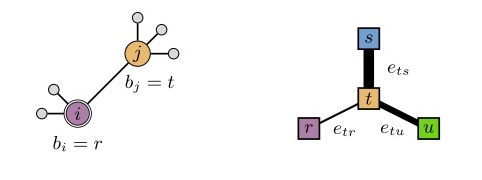
\includegraphics[width=0.9\linewidth]{pictures/topic/peixioto_move.jpg}
  \caption{Left: Local neighbourhood of node $i$ belonging to block $r$, and a randomly chosen neighbour $j$ \
  belonging to block $t$. \
  Right: Block multi-graph, indicating the number of edges between blocks, represented as the edge thickness. \
  In this example, the attempted move $bi \to s$ is made with a larger probability than either $bi \to u$\
   or $bi \to r$ (no movement), since $e_{ts}>e_{tu}$ and $e_{ts}>e_{tr}$.}
  \label{fig:topic_peixioto_move}
\end{figure}

In order to remove eventual biases due to the initial configuration the model is run with $5$ different initial states, then the final state with the minimal entropy is selected.

Once the model run it is possible to estimate the probability distribution of words inside a topic
\[P(w|t_w)=\frac{\text{\# of edges on $w$ to $t_w$}}{\text{\# of edges on $t_w$}}\]
and the topic distribution inside a document
\[P(t_w|d)=\frac{\text{\# of edges on $d$ from $t_w$}}{\text{\# of edges on $d$}}\]
This algorithm can set to have overlapping partitions; in this case, the presence of a word in a topic is not trivial and can be estimated as
\[P(t_w|w)=\frac{\text{\# of edges on $w$ to $t_w$}}{\text{\# of edges on $w$}}\]
or the presence of a document in a cluster
\[P(t_d|d)=\frac{\text{\# of edges on $d$ to $t_d$}}{\text{\# of edges on $d$}}\]

See appendix~\ref{app:hsbm} for a detailed analysis of the maths behind the algorithm and \url{https://cloud.docker.com/repository/docker/fvalle01/hsbm} for the extension of~\cite{gerlach2018network} to non-linguistics component systems datasets.


%%metrics
\section{Metrics and benchmarks}
Before running topic modelling, it is useful to define some metrics to test and benchmark the model. In particular the model searches sets on the two sides of the network the one containing samples and the one containing genes. Samples are extracted from datasets where much metadata are available, some of these metadata labels will be used to benchmark the model. To study genes enrichment test are necessary.

Looking at the samples side of the network, the outputs are sets of samples, the clusters. One can state the model works if all, or at least the majority, of samples in the same cluster share some label. Here the tissue is considered as the main label.

Note that this work's model is a non supervised one, but a ground truth is available from metadata. So every sample has a certain probability to have a certain property (the true tissue label), let's call this $P(C)$ and a certain probability of being in a cluster (model's output), let's call this $P(K)$.
It is possible to define some quantities, the homogeneity
\begin{equation}\label{eq:homogeneity}
    h=1-\frac{H(C|K)}{H(C)}
\end{equation}
defining the entropy
\begin{equation}\label{eq:hck}
    H(C|K)=\sum_{c\in \mathrm{tissues},\\ k \in \mathrm{clusters}}\frac{n_{c k}}{N}Log\left(\frac{n_{c k}}{n_k}\right)
\end{equation}
where $n_{c k}$ is the number of nodes of type $c$ in cluster $k$, $N$ the number of nodes and $n_k$ the number of nodes in cluster $k$. It is evident that if all nodes inside cluster $k$ are of the same type $c$ $n_{c k}=n_{k}$, $H(C|K)=0$ and $h=1$, it is actually a complete homogeneous situation.

Another quantity can be defined: the so-called completeness
\begin{equation}\label{eq:completness}
    c=1-\frac{H(K|C)}{H(K)},
\end{equation}
$H(K|C)$ is defined in the same way as~\ref{eq:hck}. Completeness measures how well nodes of the same type are distributed in the same cluster.

Ideally one wants a method which output is both homogeneous and complete. So it is possible to define the V-measure as the harmonic average of the two:
\begin{equation}\label{eq:mutualinformation}
    \mathrm{V-measure}=2\frac{h c}{h + c},
\end{equation}
which is actually the normalized mutual information between $P(C)$ and $P(K)$~\cite{rosenberg2007v}. Please refer to appendix~\ref{app:vmeasure} for the detailed maths. In figure~\ref{fig:topic/metric_scores_primarysite} an example of the V-measure score estimated at the different layers of the hierarchy; note that the number of clusters increases going deeper in the hierarchy. In the same figure homogeneity and completeness are reported, note that with few clusters the situation is more complete, but when the number of clusters increases completeness goes down and homogeneity increases. 
\begin{figure}[htb!]
    \centering
    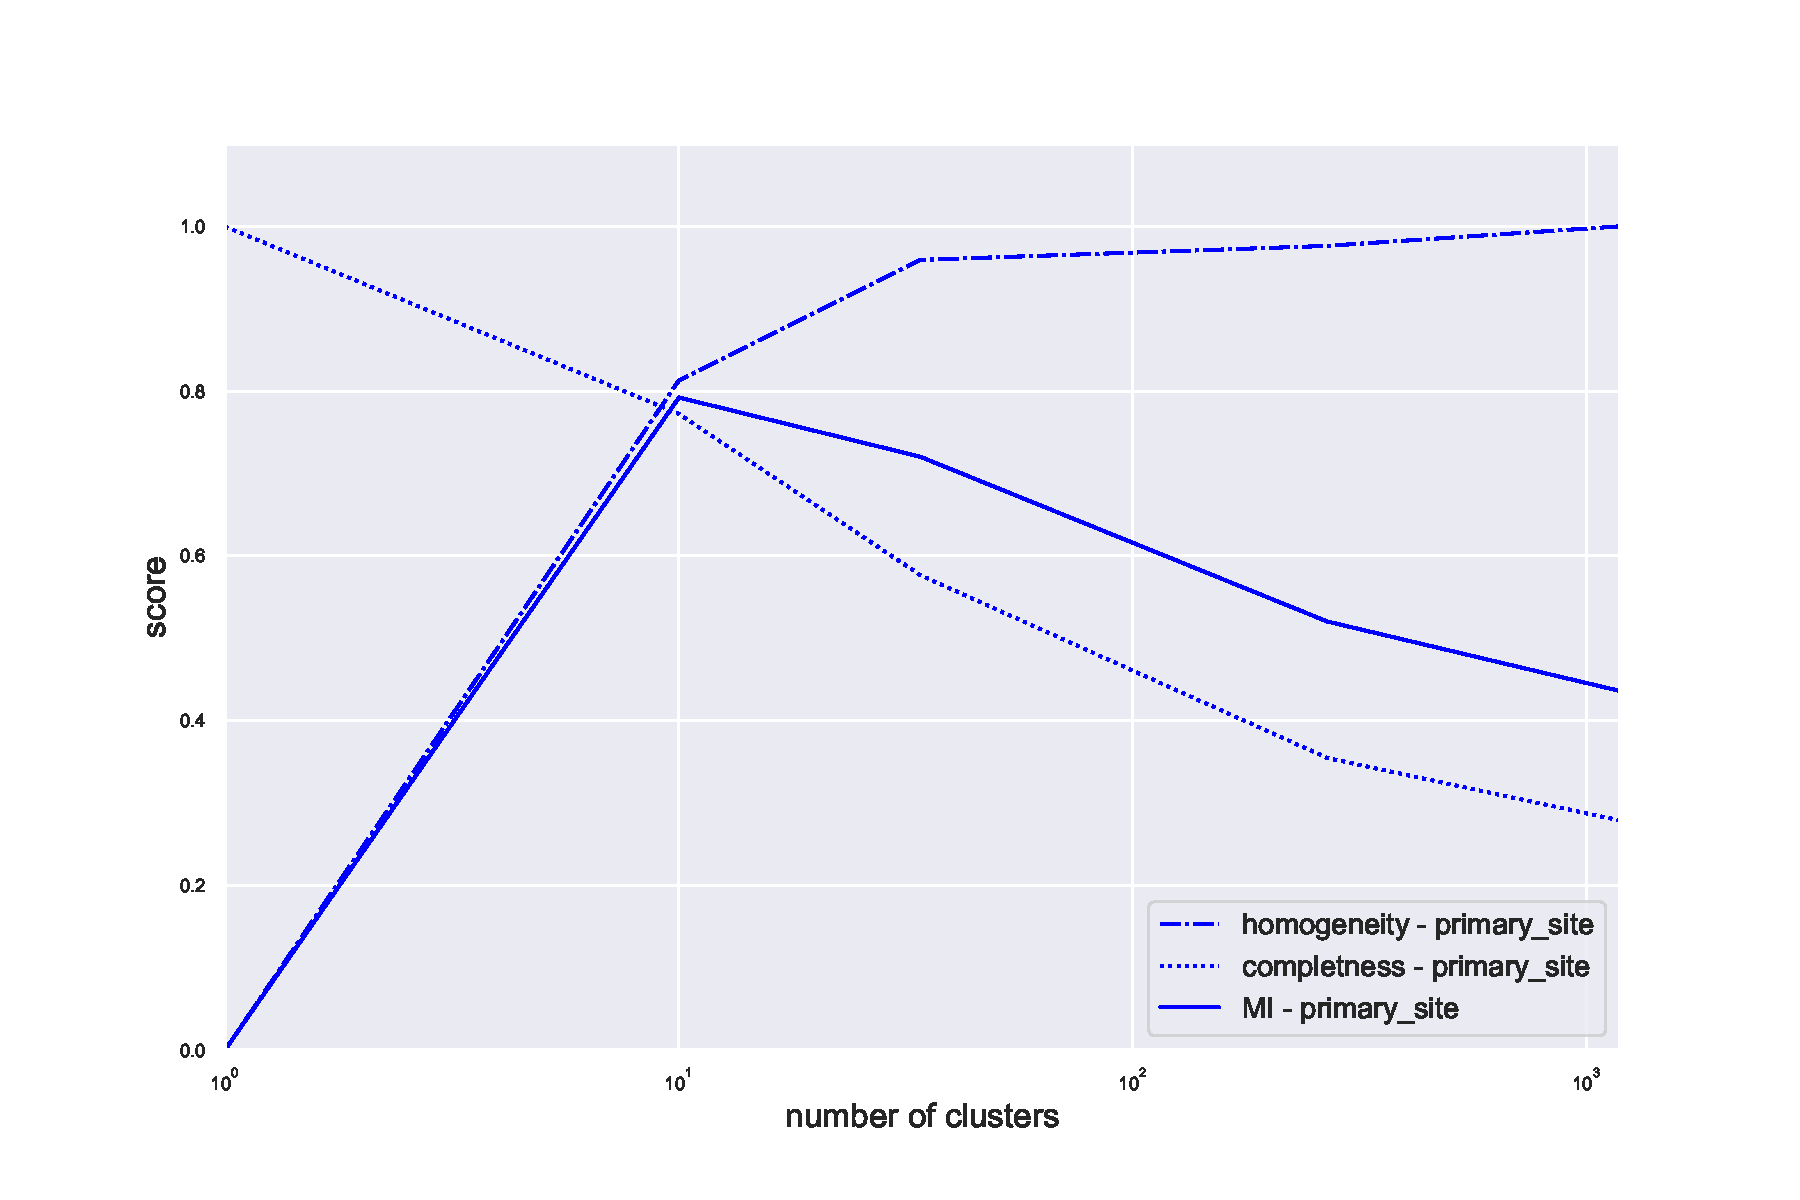
\includegraphics[width=0.8\linewidth]{pictures/topic/gtex/oversigma_10tissue/metric_scores_primarysite.pdf}
    \caption{Score across hierarchy. The V-measure or normalized mutual information MI is the harmonic average between homogeneity and completeness.}
    \label{fig:topic/metric_scores_primarysite}
\end{figure}

In the next sections will be studied also the maximum fraction of label in the same cluster defined as 
\[\mathrm{max}_{c\in k}\frac{n_{c k}}{n_k}.\] Also the number of different labels in the same cluster will be studied.
\FloatBarrier

%%preprocess
\section{Pre-process}
To make the algorithm faster, it could be useful to do a pre-processing of the data.
Different approaches were tested, all of them involving the quantities defined in~\ref{ch:structure}. The goal is to identify components which are able to best separate the realizations. 
\paragraph{Low occurrence genes} were selected firstly to approach topic modelling. A $0.5$ threshold was set on occurrence. This method selects genes that appears (have expression greater than zero) only in less than half samples. This approach has some limitations, for instance it doesn't consider genes that appear everywhere (with occurrence $\simeq 1$) but changes their behaviour across realisations.

\paragraph{tf-idf (term frequency–inverse document frequency)} should help. This approach doesn't take in account original expression values $n_{ij}$, but a transformed version
\[
n^{new}_{ij}=\frac{n_{i j}}{M_j}\times \left(1-Log\left(o_i\right)\right)
\] which increases the importance of components with small occurrence $o_i$. This approach doesn't actually select components, which is still an issue.

\paragraph{Highly variable} genes can be selected. This is done using the $CV^2$ analysis done in chapter~\ref{ch:scalinglaws}.
\begin{figure}[htb!]
    \centering
    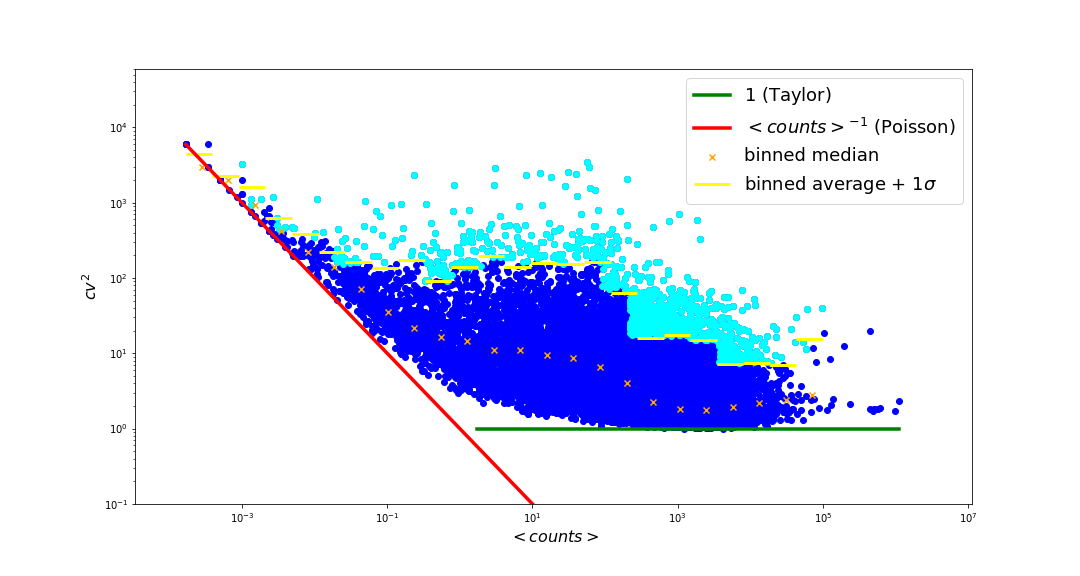
\includegraphics[width=0.8\linewidth]{pictures/topic/cvmean_oversigma.png}
    \caption{Highly variable genes}
    \label{fig:topic/cvmean_oversigma}
\end{figure}
Plotting the coefficient of variation versus the mean for each component reveals which components have higher variance with respect to components which, on average, have a similar behaviour. Binned averages and variances were estimated, and only genes with a $CV^2$ over a $\sigma$ greater than the bin's mean were considered. This method seems to select useful genes even if the binned average bound is quite noisy.

\paragraph{Distance from boundaries} can be a similar and alternative method to select highly variable genes. In this case the bound is smooth and well defined.
\begin{figure}[htb!]
    \centering
    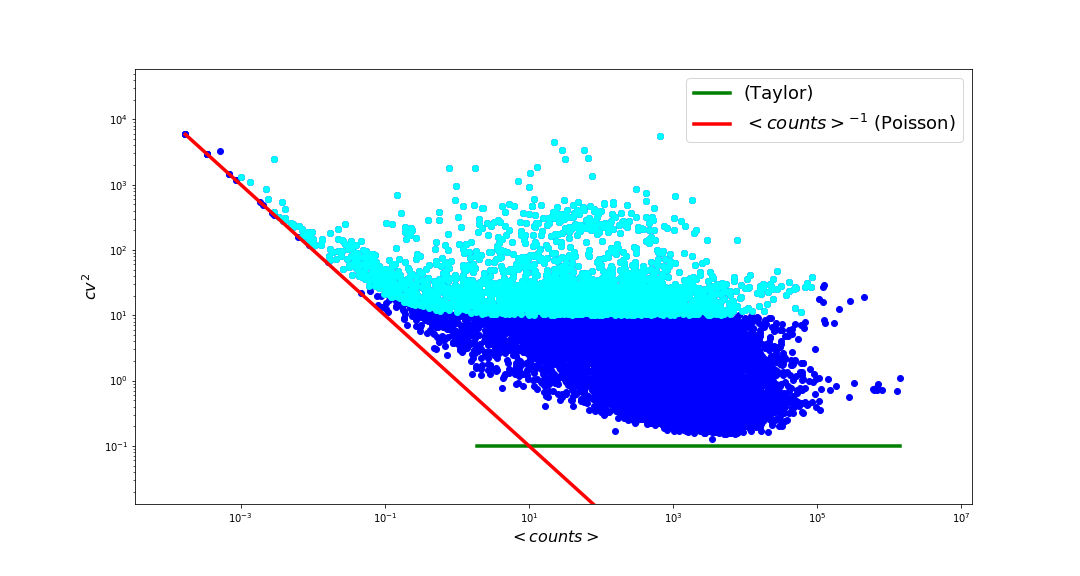
\includegraphics[width=0.8\linewidth]{pictures/topic/cvmean_oversampling.png}
    \caption{Genes distant from the boundaries}
    \label{fig:topic/cvmean_oversampling}
\end{figure}
The distribution as discussed in~\ref{ch:scalinglaws} have a Poisson-like and a Taylor-like boundaries. So can be considered only components that are the most distant from these boundaries. Moreover this boundaries can be found with a simple null model, as shown in figure~\ref{fig:scaling/gtex/cvmean_loglog_sampling} the sampling model defines the lower bound of the data.

The last two approaches are the ones which lead to better results, in the following sections gene selection was done by getting only highly variables genes.

\section{Run on GTEx}
\draft{Firstly the algorithm is run on a subset of $5$ tissues of GTEx}
\draft{metti 5 tissues?}
\begin{figure}[htb!]
    \centering
    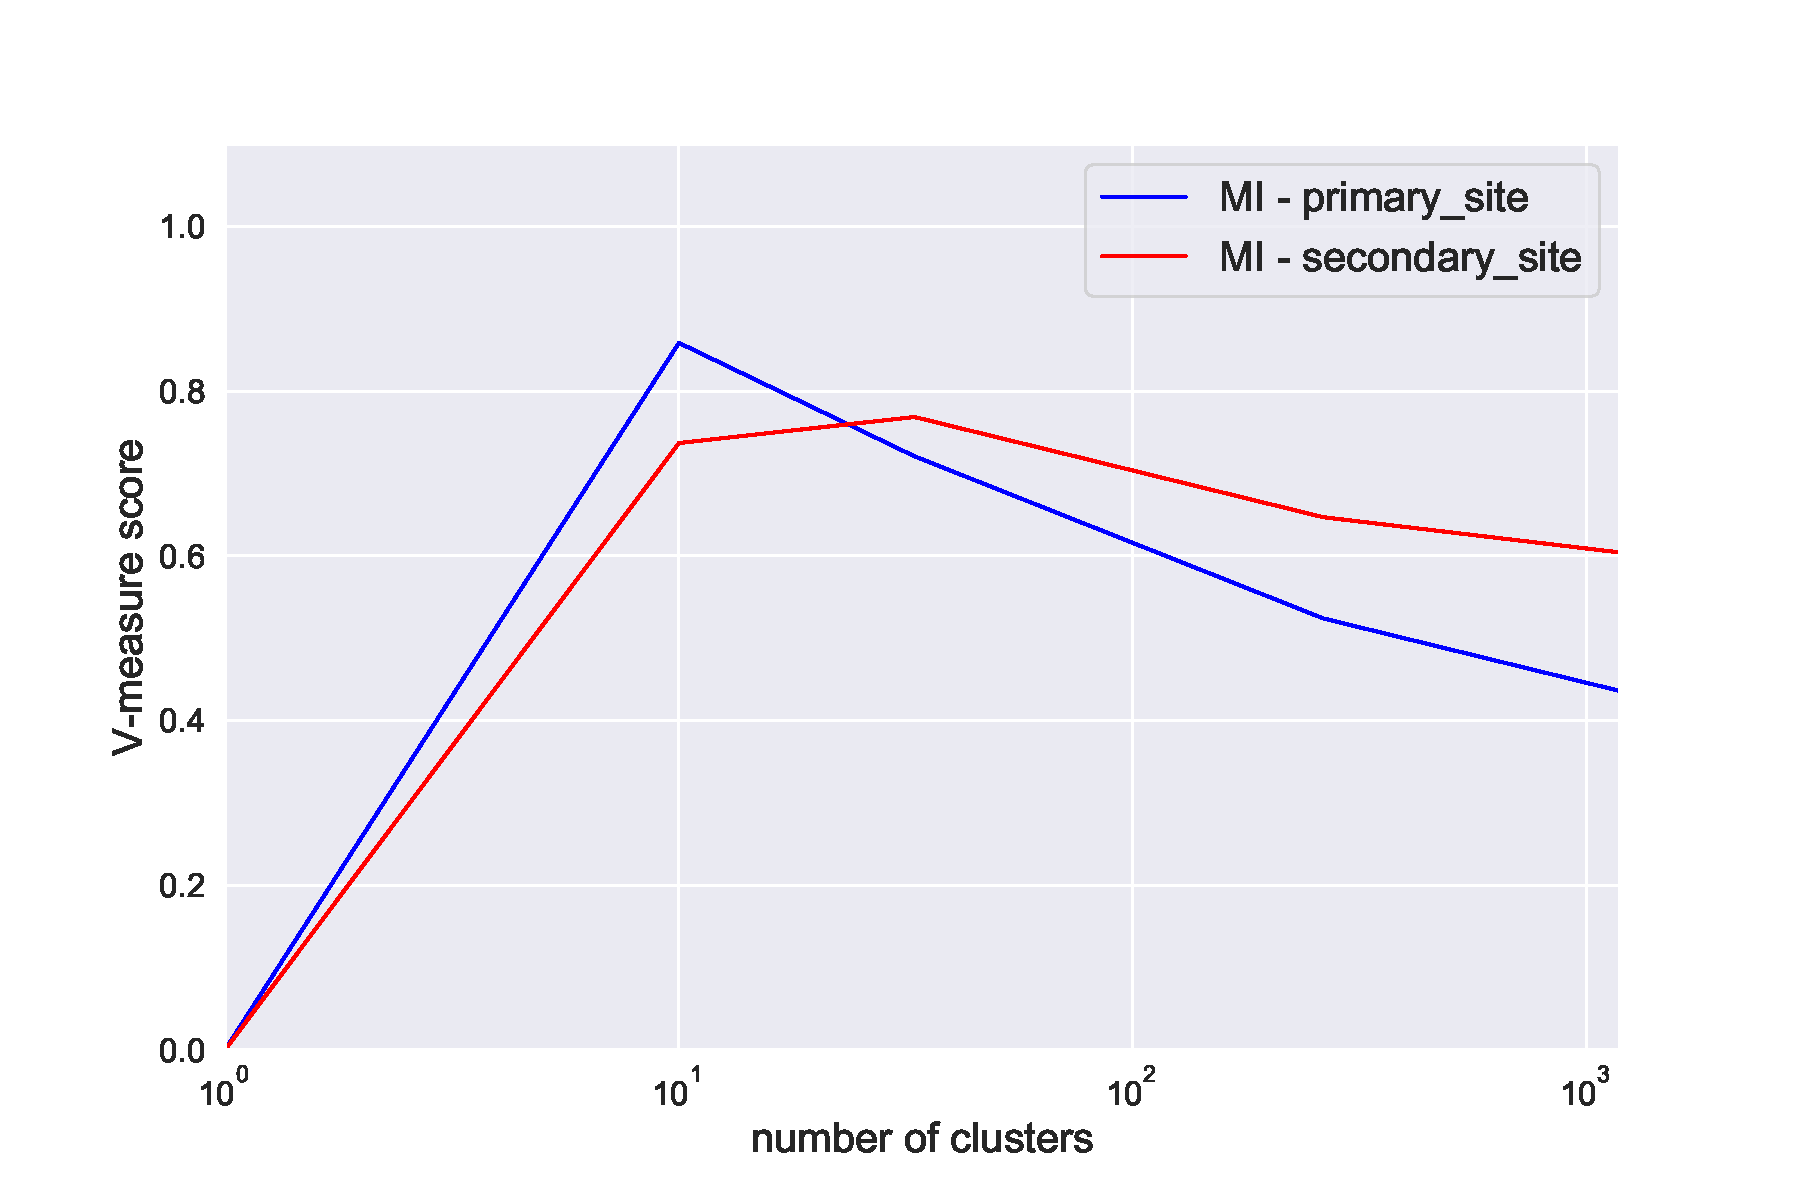
\includegraphics[width=0.9\linewidth]{pictures/topic/gtex/oversigma_10tissue/metric_scores.pdf}
    \caption{Scores accross hierarchy}
    \label{fig:my_label}
\end{figure}

\begin{figure}[htb!]
    \centering
    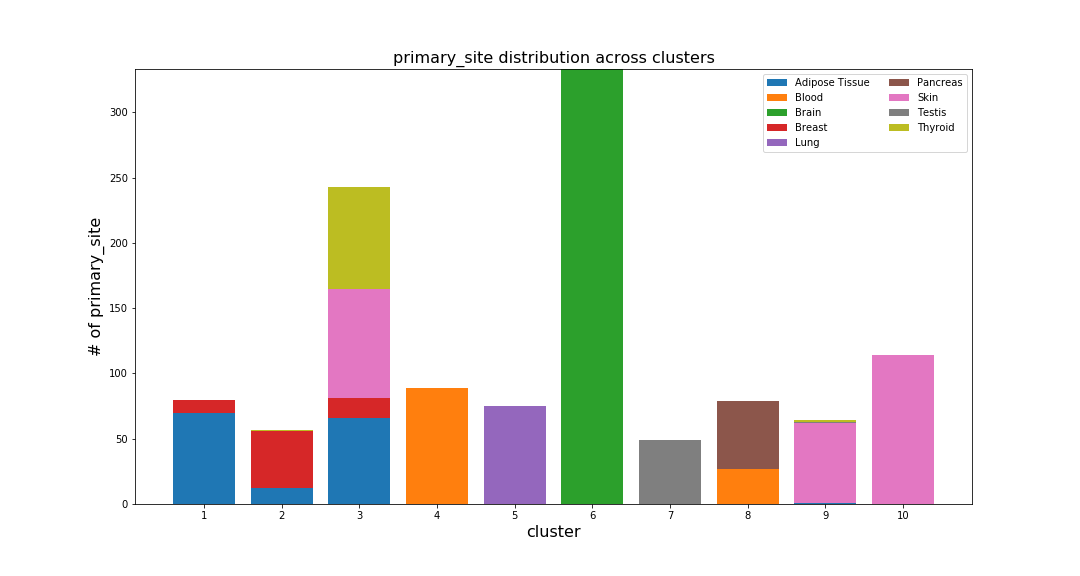
\includegraphics[width=0.9\linewidth]{pictures/topic/gtex/oversigma_10tissue/clustercomposition_l3_primary_site.png}
    \caption{Caption}
    \label{fig:topic/gtex/oversigma_10tissue/clustercomposition_l2_primary_site}
\end{figure}

\begin{figure}[htb!]
    \centering
    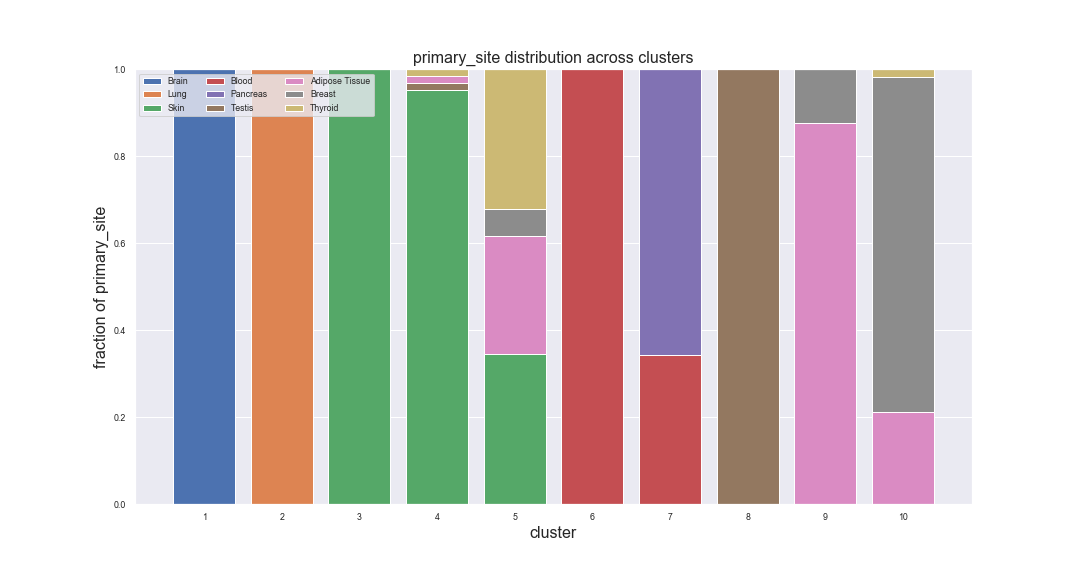
\includegraphics[width=0.9\linewidth]{pictures/topic/gtex/oversigma_10tissue/fraction_clustercomposition_l3_primary_site.png}
    \caption{Caption}
    \label{fig:topic/gtex/oversigma_10tissue/fraction_clustercomposition_l2_primary_site}
\end{figure}

\begin{figure}
    \centering
    \begin{minipage}{0.45\textwidth}
    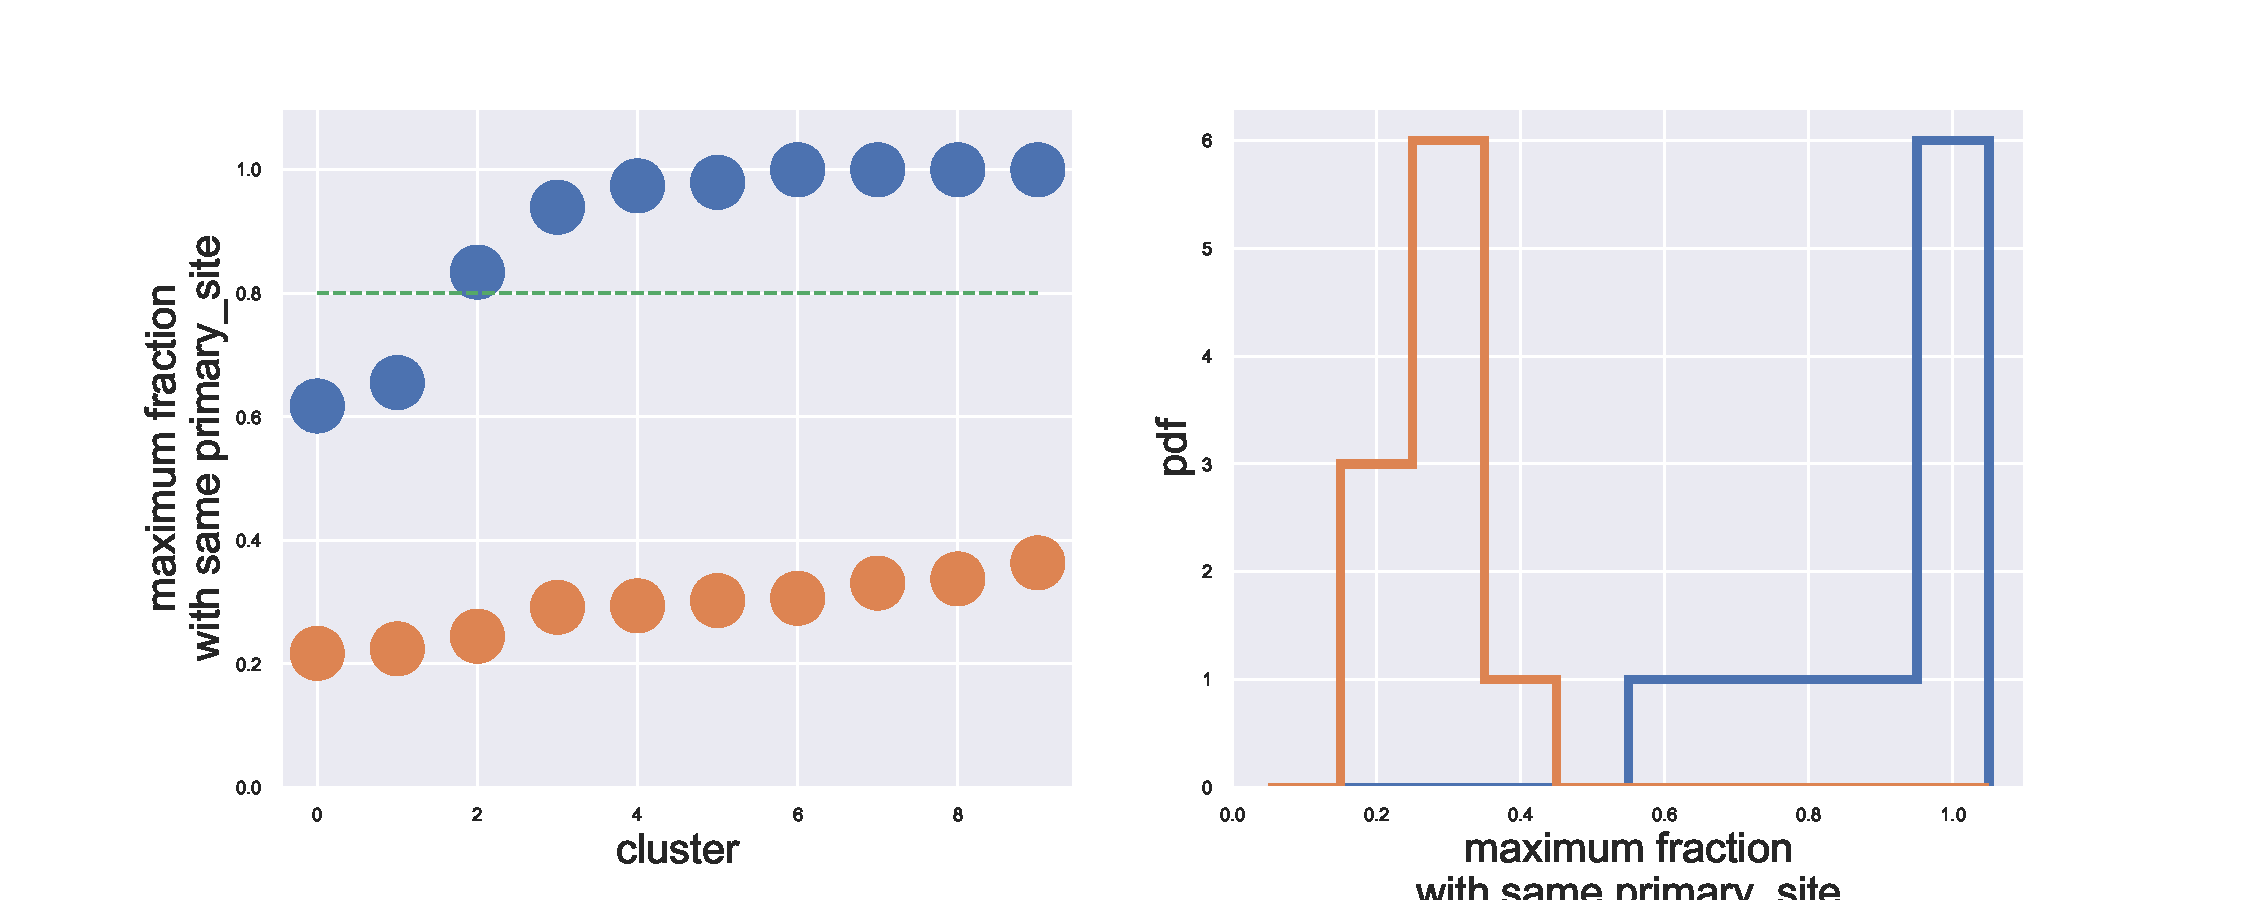
\includegraphics[width=0.9\linewidth]{pictures/topic/gtex/oversigma_10tissue/shuffledcluster_maximum_l3_primary_site.pdf}
    \end{minipage}
    \hspace{3mm}
    \begin{minipage}{0.45\textwidth}
    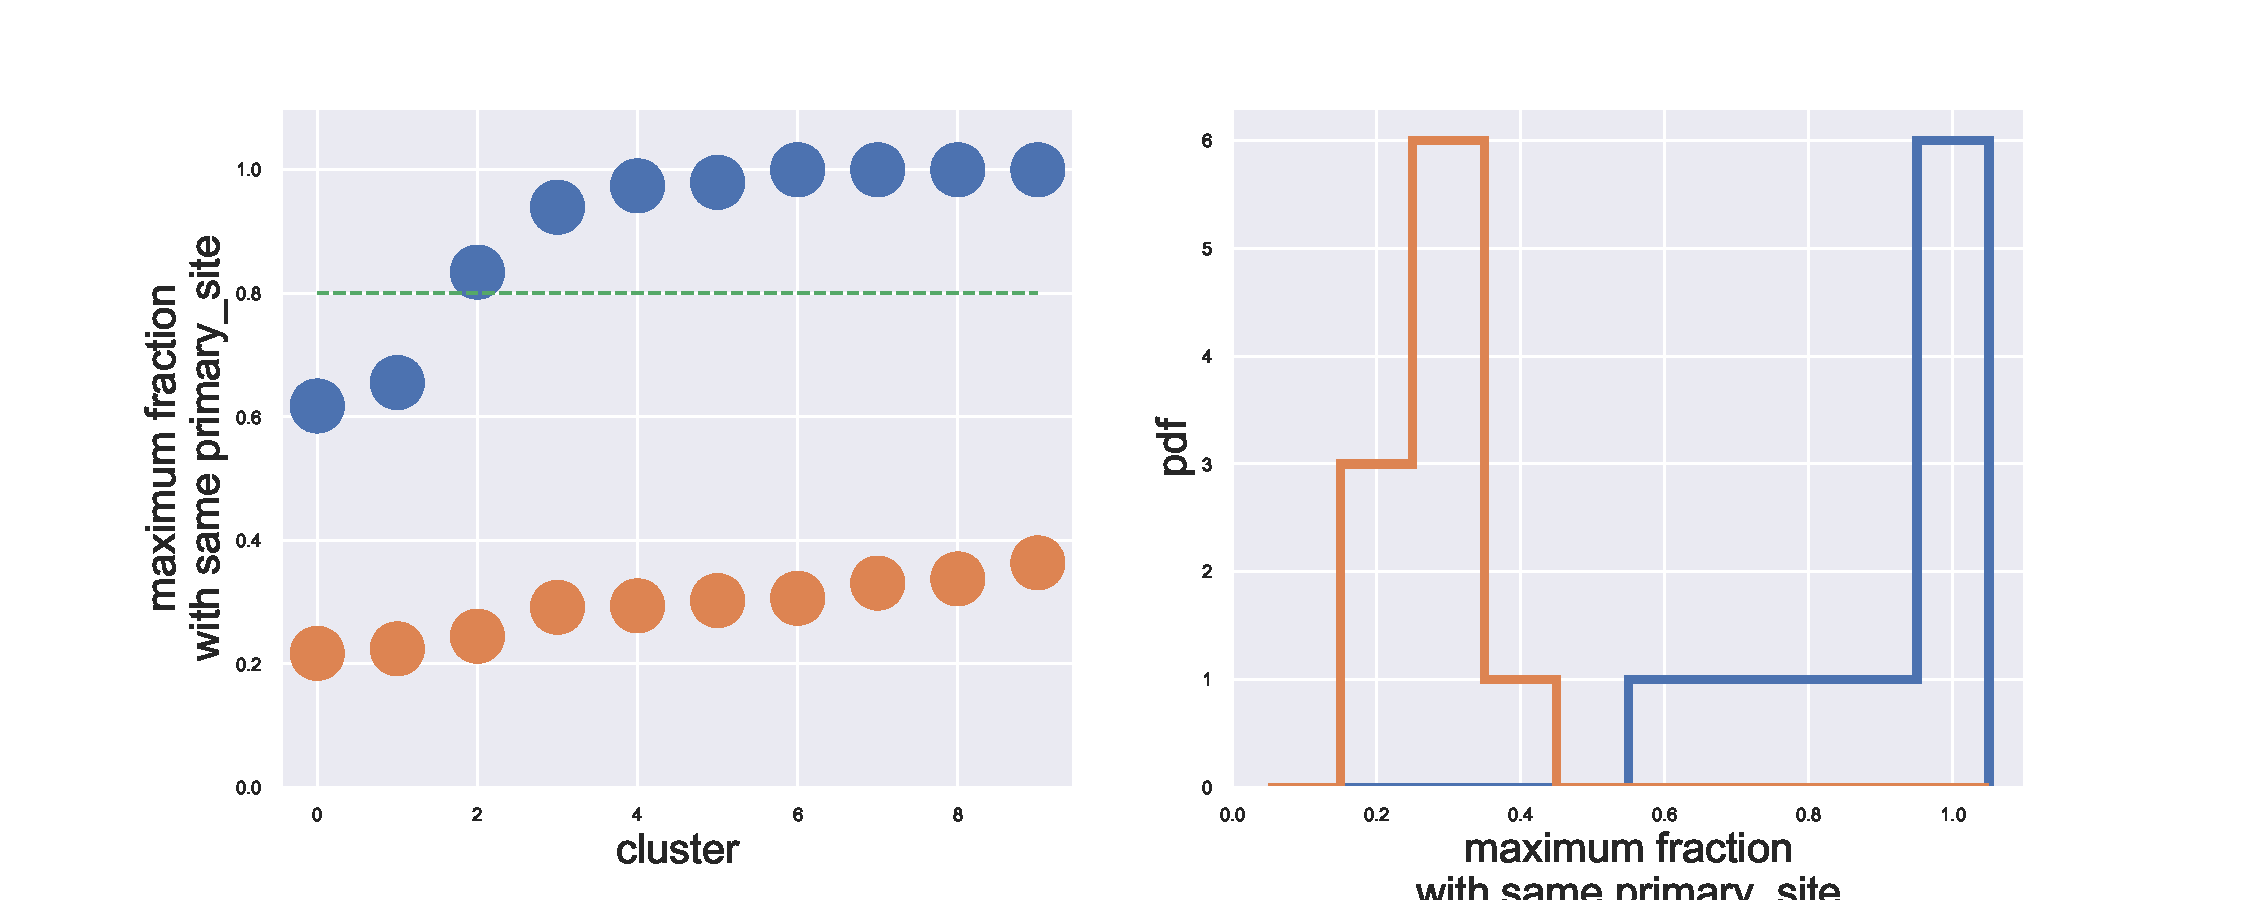
\includegraphics[width=0.9\linewidth]{pictures/topic/gtex/oversigma_10tissue/shuffledcluster_maximum_l3_primary_site.pdf}
    \end{minipage}
    \\
    \begin{minipage}{0.45\textwidth}
    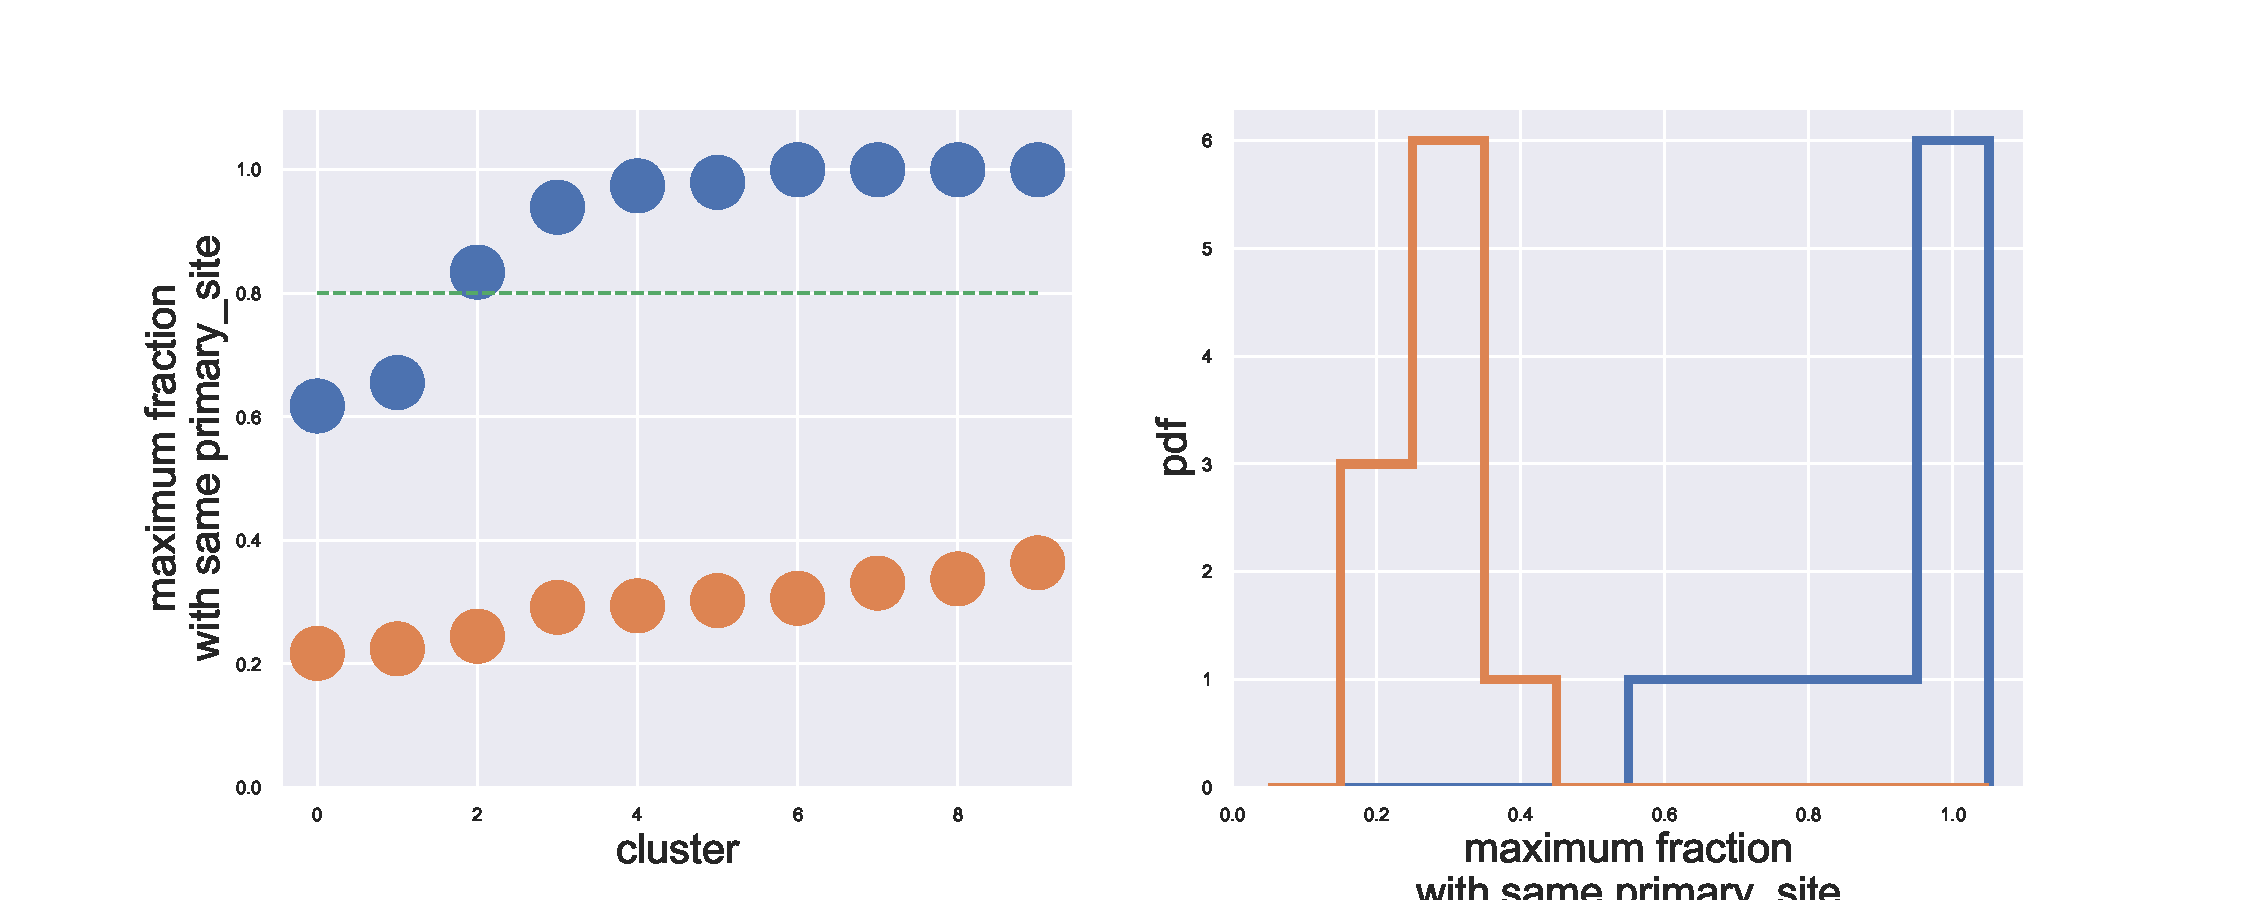
\includegraphics[width=0.9\linewidth]{pictures/topic/gtex/oversigma_10tissue/shuffledcluster_maximum_l3_primary_site.pdf}
    \end{minipage}
    \hspace{3mm}
    \begin{minipage}{0.45\textwidth}
    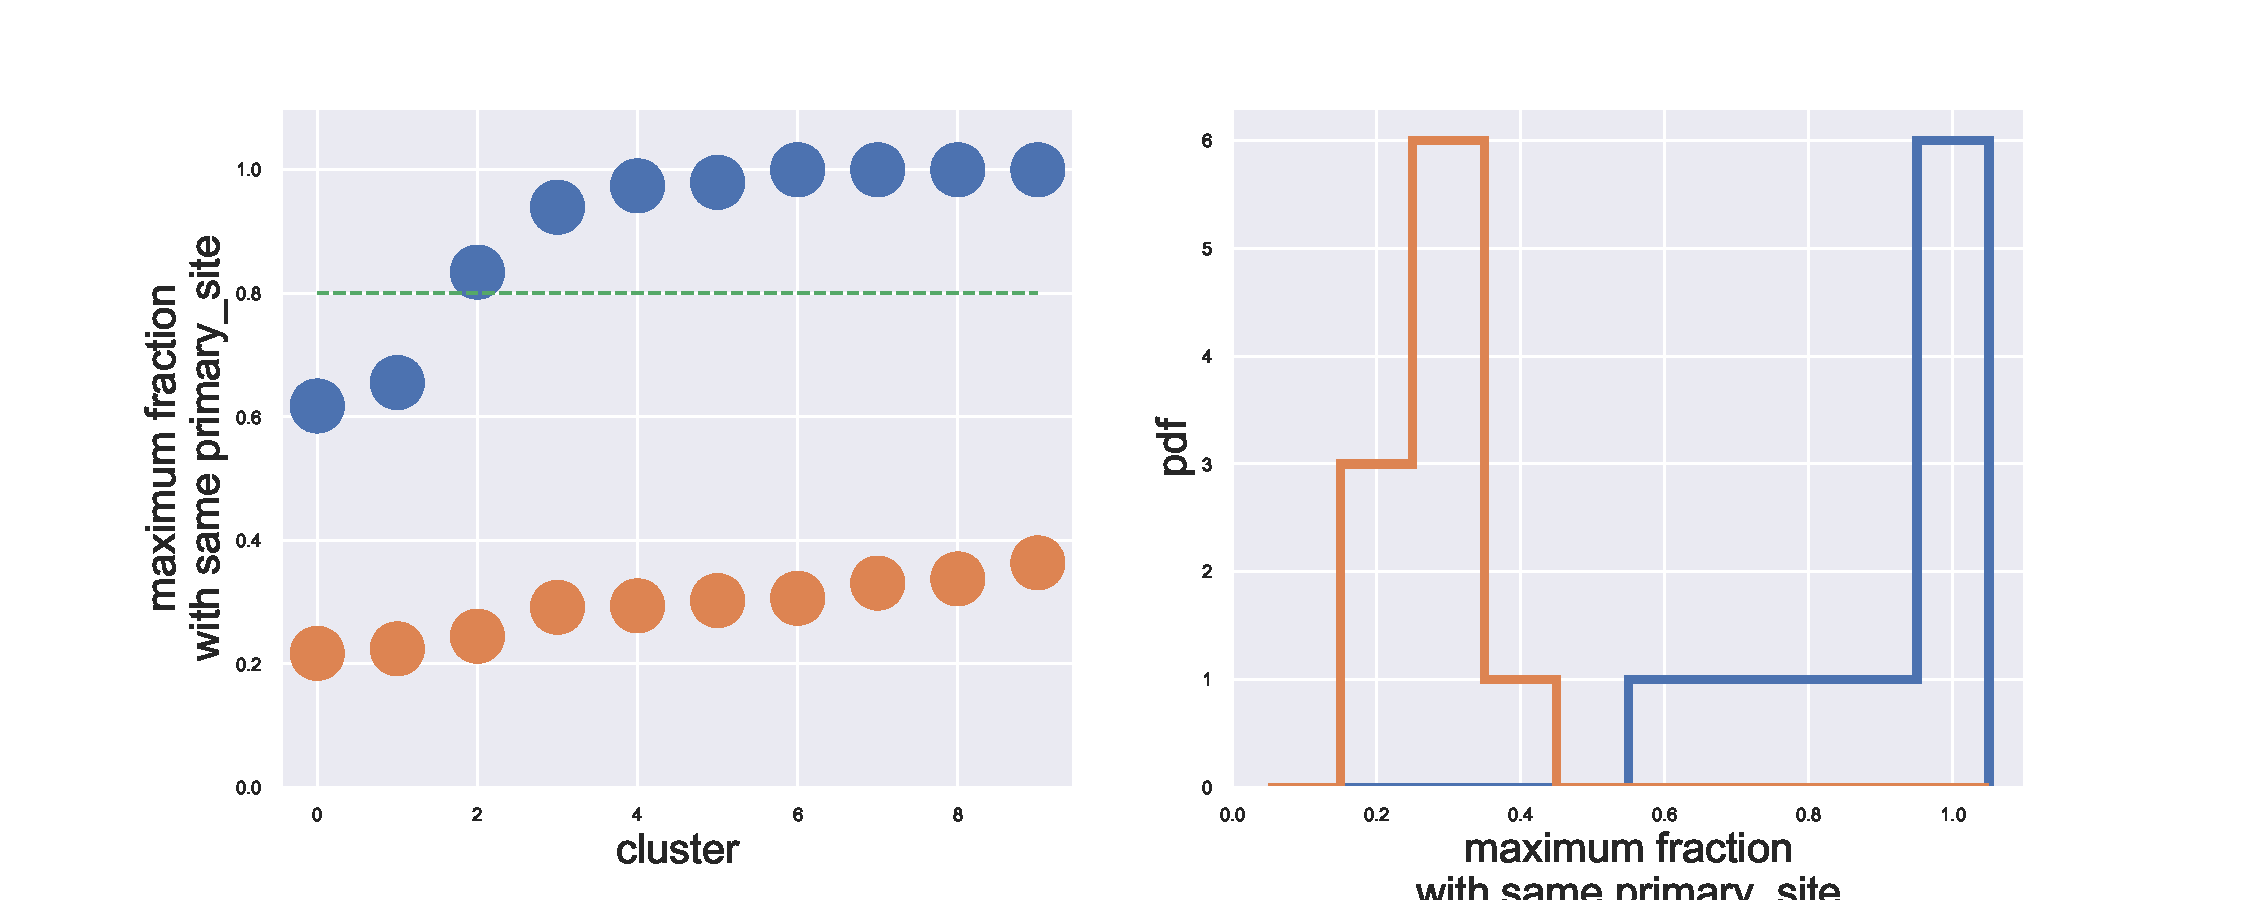
\includegraphics[width=0.9\linewidth]{pictures/topic/gtex/oversigma_10tissue/shuffledcluster_maximum_l3_primary_site.pdf}
    \end{minipage}
\end{figure}


\begin{figure}[htb!]
    \centering
    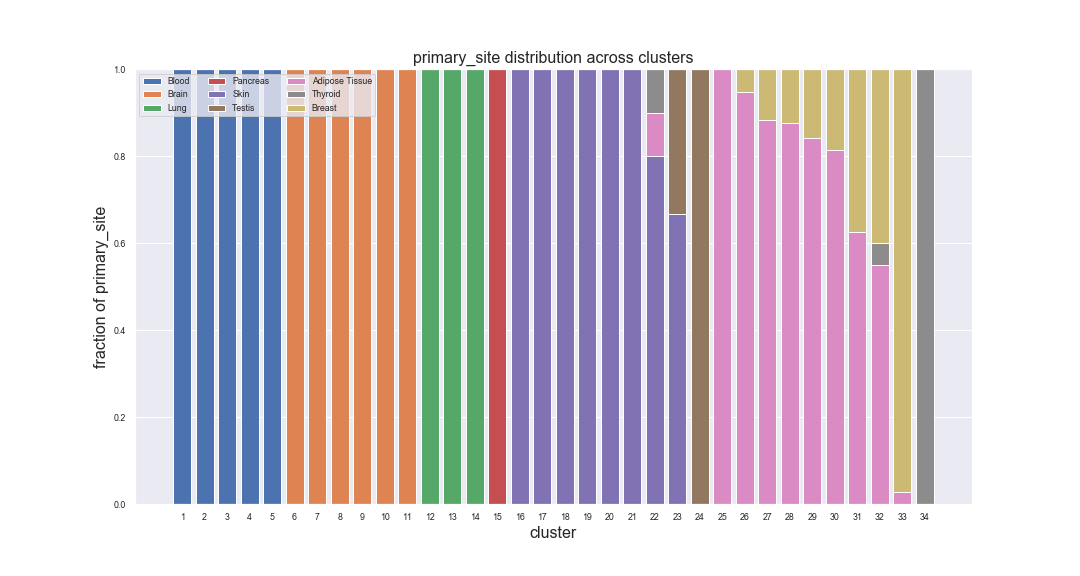
\includegraphics[width=0.9\linewidth]{pictures/topic/gtex/oversigma_10tissue/fraction_clustercomposition_l2_primary_site.png}
    \caption{Caption}
    \label{fig:topic/gtex/oversigma_10tissue/fraction_clustercomposition_l2_primary_site}
\end{figure}

\begin{figure}[htb!]
    \centering
    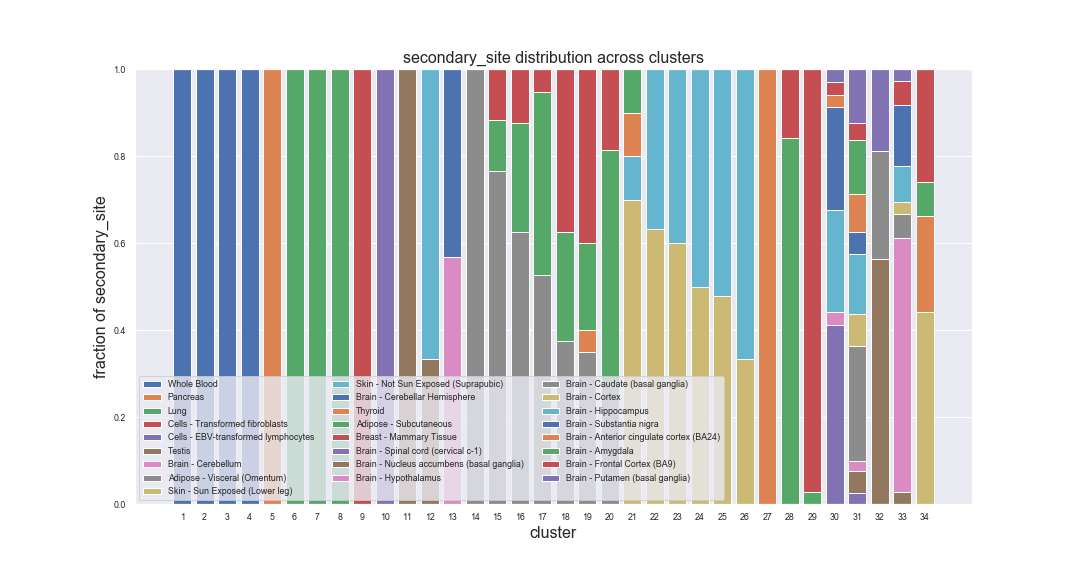
\includegraphics[width=0.9\linewidth]{pictures/topic/gtex/oversigma_10tissue/fraction_clustercomposition_l2_secondary_site.png}
    \caption{Caption}
    \label{fig:topic/gtex/oversigma_10tissue/fraction_clustercomposition_l2_secondary_site}
\end{figure}


Using as gene set ~\cite{Ardlie2015} enrichment test can be made \cite{Kuleshov2016}

Enrichment test are made once for each topic, starting from the layer with more genes per 
single topic. Test are made across multiple categories.

\section{Run on TCGA}

\section{Mixed runs}

\draft{hierarchical clustering}
\draft{This is better than LDA because...}